%%%%%%%%%%%%%%%%%%%%%%%%%%%%%%%%%%%%%%%%%%%%%%%%%%%%%%%%%%%%%%%%%%%%%%%%%%%%%%%%
%								CHARAC PROPAL								   %
%%%%%%%%%%%%%%%%%%%%%%%%%%%%%%%%%%%%%%%%%%%%%%%%%%%%%%%%%%%%%%%%%%%%%%%%%%%%%%%%
So far we have shown that the \gls{jacob} of an optimal model \(\jac{\MLmodel^\star}{\xxx}\) may emphasize \glspl{poi}.
In practice however, the evaluator does not have access to the optimal model, but a trained estimation of it, denoted by \(\MLmodel(\cdot, \MLparam)\).
Here we follow this idea in contexts where the approximation is modeled by training \glspl{dnn}.
\autoref{sec:grads_nn} explains how to compute the gradient visualization and the \gls{jacob} based on a trained \gls{dnn}.
\autoref{sec:toy_example} illustrates our claim with a toy example.
Finally, \autoref{sec:related_works} is dedicated to the comparison of our approach with state-of-the-art methods for leakage characterization.


\subsection{Gradient Approximation with Neural Networks}
\label{sec:grads_nn}
In \autoref{sec:universal_approx_thm} we recalled that the universal approximation theorem allows to accurately approximate any function with a \gls{mlp}, up to a precision depending on the number of neurons in the intermediate layers.
It turns out that this theorem also holds for the derivatives of the function to approximate: the latter ones can be accurately approximated by the derivatives of the approximating \gls{mlp}~\cite{hornik_approximation_1991}.%
\footnote{
	The interested reader may refer to the survey of Pinkus~\cite[Sec.~4]{pinkus_approximation_1999}.
}
Hence, the \gls{jacob} of a trained \gls{dnn}, \ie{} \(\jac{\MLmodel(\cdot, \MLparam)}{\xxx}\) represents a sound surrogate to the \gls{jacob} of the optimal model \(\MLmodel^\star\).

To accurately and efficiently compute the \gls{jacob} of a \gls{dnn}, the backprop algorithm presented in \autoref{sec:computing_gradient} can be used.
Originally, it applies a reverse mode differentiation in order to compute the gradient of the loss function with respect to the parameter vector \(\MLparam\).
Interestingly, we explained that the backward pass of the reverse mode actually computes the derivatives of each layer function with respect to each of its inputs, even if the latter ones are not explicitly part of the learning parameters.
This particularly concerns the very first layer which takes as inputs not only some learning parameters but also the input trace \(\xxx\).
In other words, given an input trace \(\xxx\), its corresponding sensitive value \(\z\), and the loss function used for the optimization \(\ell: \probSet{\sensVarSet} \times \sensVarSet \rightarrow \realSet_+\),%
\footnote{
	See a definition in \autoref{eq:loss_function}.
}
it is possible to compute for free the gradient of \(\lossFunc{\MLmodel(\xxx, \MLparam), \z}\) with respect to the input trace \(\xxx\) whenever the gradient of \(\lossFunc{\MLmodel(\xxx, \MLparam), \z}\) with respect to the learning parameters \(\MLparam\) is required.
As a consequence, computing such a gradient can be done with a negligible overhead during an iteration of the \gls{sgd}.

Actually, we justified when presenting the backprop algorithm in \autoref{sec:computing_gradient} that the modern \gls{dl} libraries~\cite{pytorch_2019,tensorflow2015-whitepaper} are optimized to directly compute the gradient of the loss function without explicitly computing the \gls{jacob} \(\jac{\MLmodel(\cdot, \MLparam)}{\xxx}\).
However, our ultimate goal is still to know the \gls{jacob} of the \gls{dnn} model.
Hopefully, studying either the latter one or the gradient of the loss function is fairly equivalent, as one coordinate of the loss function gradient is a function of elements from the corresponding column in the \gls{jacob}, according to \autoref{lemma:chaining_rule}:
\begin{eqnarray}
	\grad[\xxx]{\lossFunc{\MLmodel(\xxx, \MLparam), \sensValue}} & = &
	\jac{\MLmodel(\cdot, \MLparam)}{\xxx}^\intercal \cdot \nabla_{\vNNOutput}\lossFunc{\MLmodel(\xxx, \MLparam),
	\sensValue} \enspace .
\end{eqnarray} 
That is why we propose to visualize the gradient of the loss function, computed with respect to the input trace, to characterize \glspl{poi} in the context of a \gls{dnn} attack, instead of the \gls{jacob} -- unless explicit mention. 
More precisely, we visualize the absolute value of each coordinate of the gradient  in order to get the sensitivity magnitude. 
In the following, such a method is named \glsfirst{gv}.
One of the advantage of this method is that the additional source code required to implement this method is very light, as shown in \autoref{fig:gv_pytorch}.

\begin{figure}
	\centering
	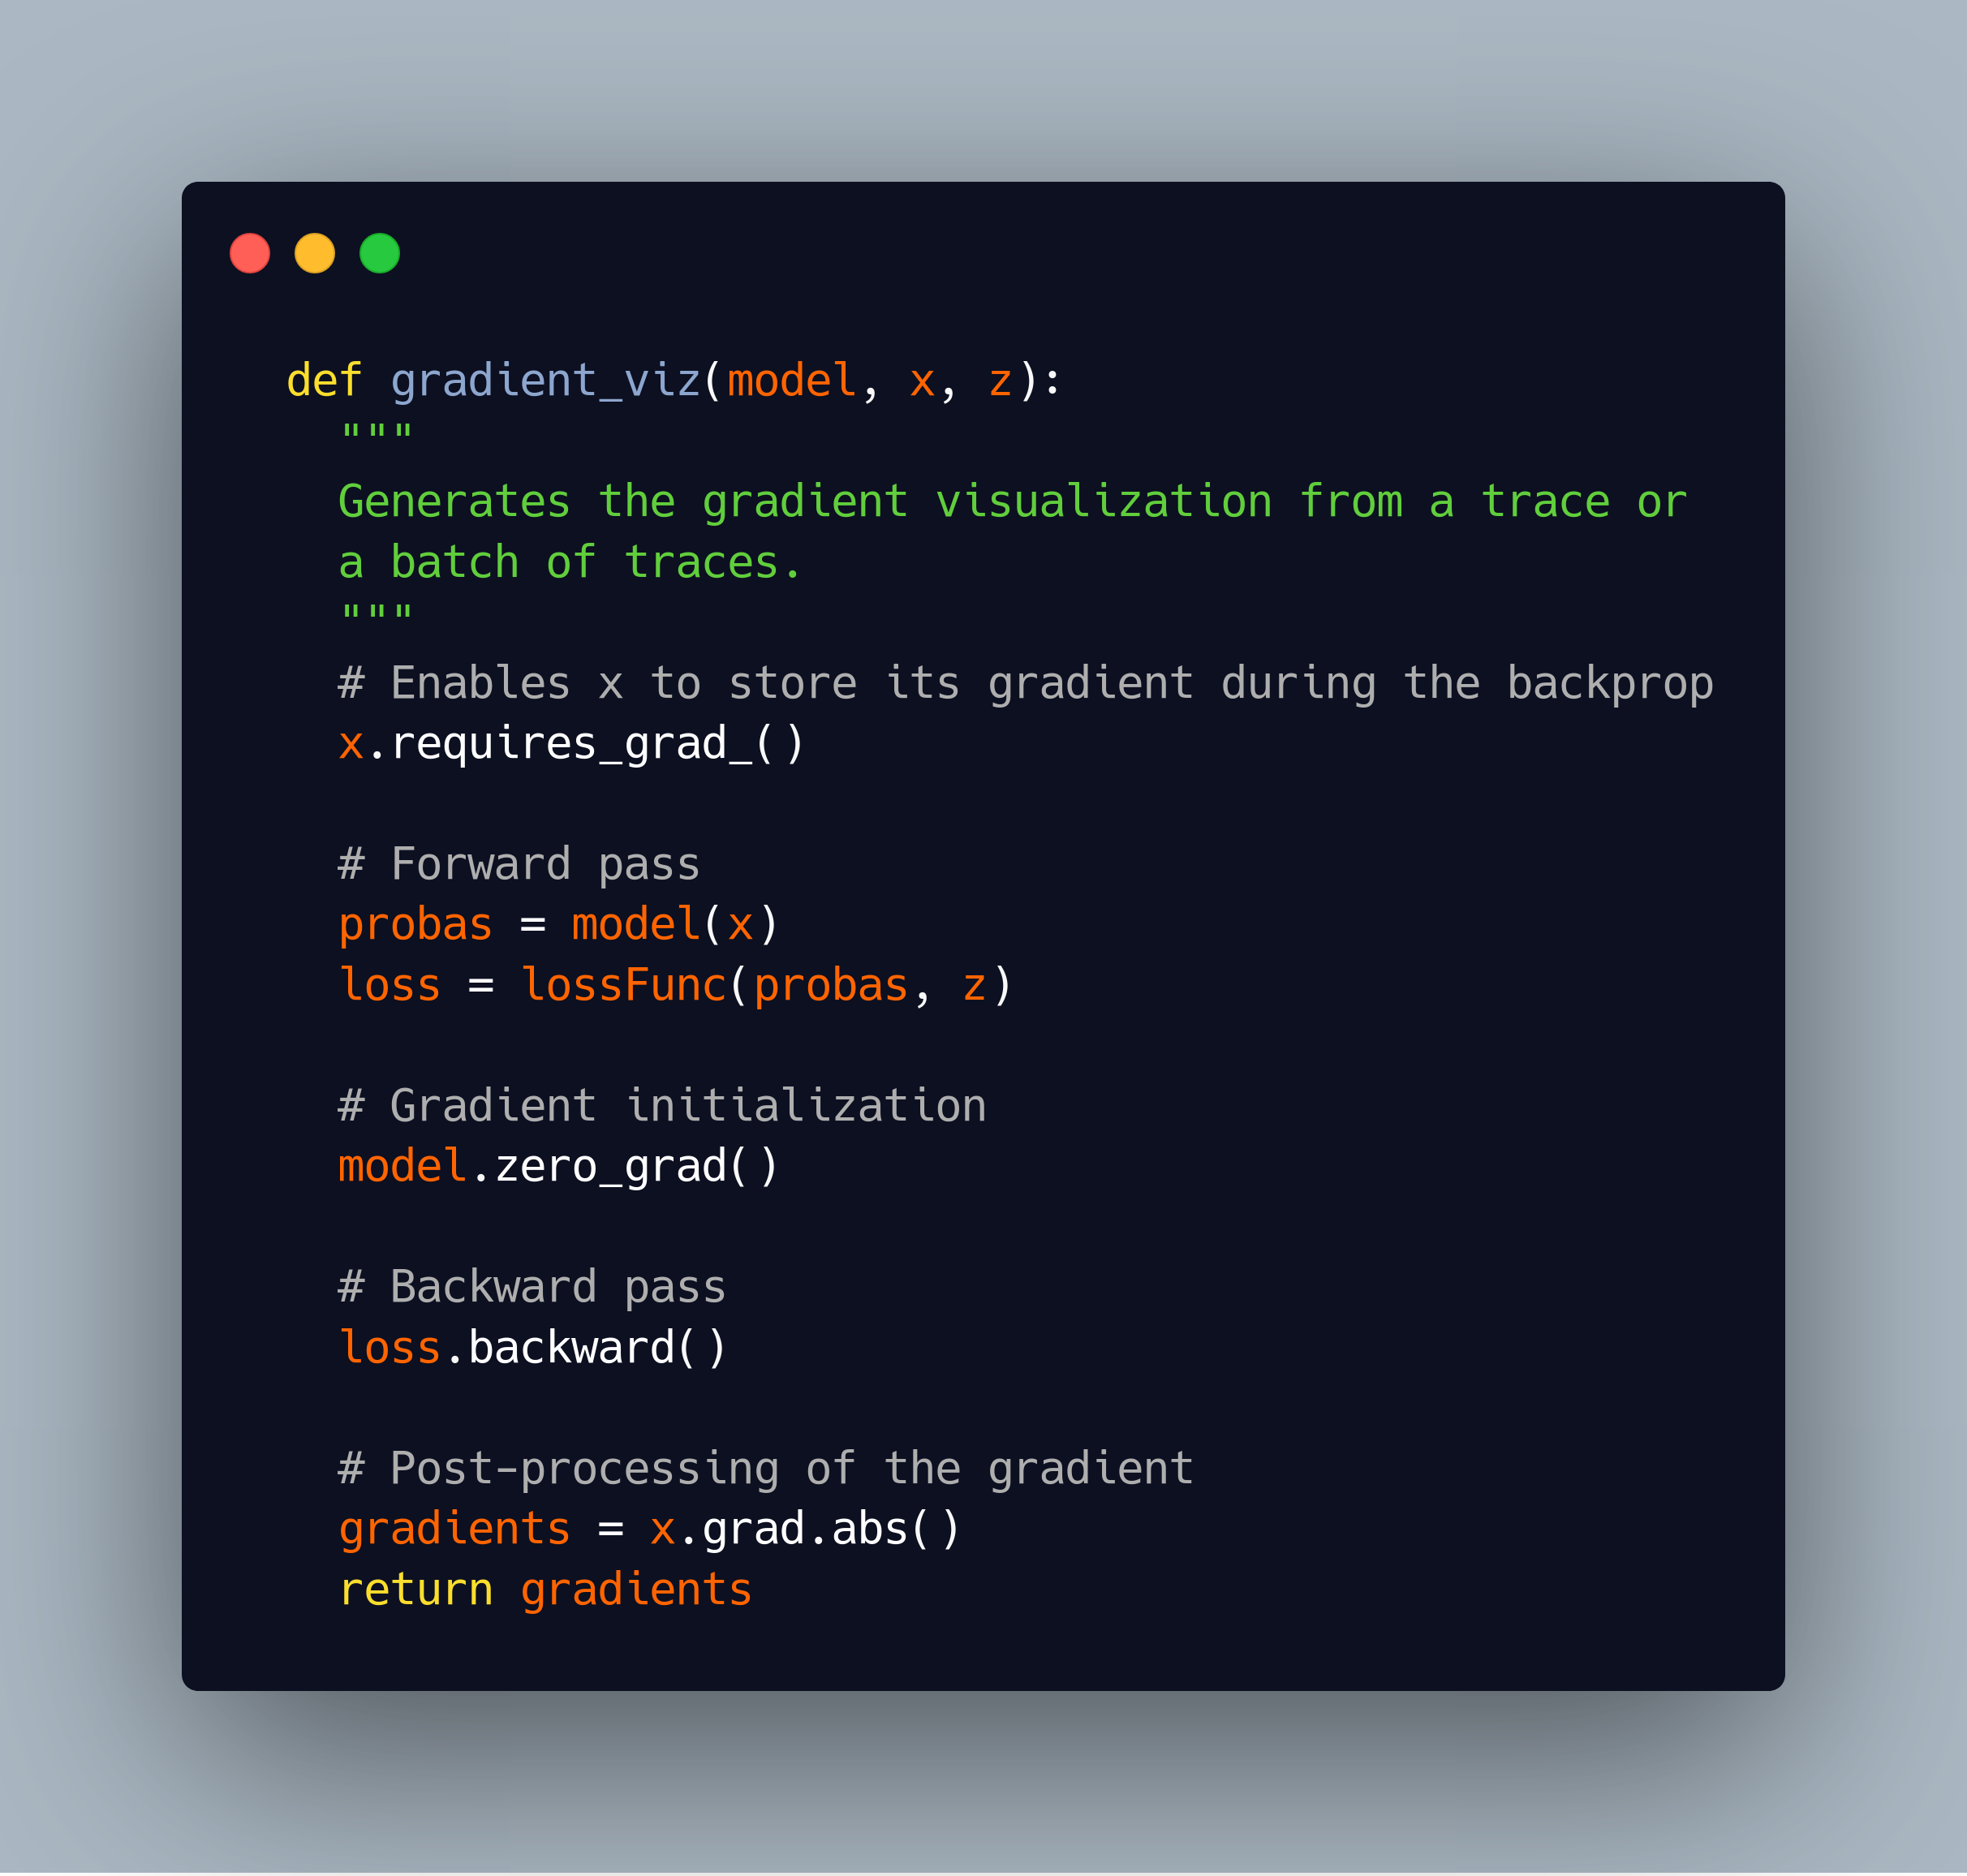
\includegraphics[width = 0.7 \textwidth]{figures/Illustrations/code}
	\caption{Source code to implement the \gls{gv} in \textsf{Pytorch}.}
	\label{fig:gv_pytorch}
\end{figure}

\subsection{Example on Simulated Data}
\label{sec:toy_example}
To illustrate and explain the relevance of the \gls{gv} method, and before going on experimental data, we here propose to apply it on a toy example, aiming at simulating simple \(\traceLength\)-dimensional leakages from an \(n\)-bit sensitive variable \(\Z\).
The method follows the same procedure as already explained in \autoref{sec:settings}.
The traces are defined such that for every \(t \in \llbracket1, \traceLength\rrbracket\):
\begin{equation}
	\xxx_i[t] =
	\begin{cases}
		u_i + b_i \mbox{, if } t \notin \{t_1, \ldots, t_{\order+1}\} \\
		\hWeight(\z_{t,i}) + b_i \mbox{ otherwise}
	\end{cases}
	\enspace ,
\end{equation}
where \((u_i)_i, (b_i)_i\) and all \((\z_{t,i})_i\) are \gls{iid} draws from the following independent random variables.
Respectively, \(\randVar{U} \sim \mathcal{B}(n, 0.5)\), \(\randVar{B} \sim \mathcal{N}(0, \sigma^2)\),%
\footnote{
	It is recalled that \(\hWeight\) denotes the Hamming weight function, see \autoref{sec:cpa}.
} 
where  and where \((\z_{1,i}, \ldots, \z_{\order+1,i})\) is a \((\order+1)\)-sharing of \(\z_i\) for the bit-wise addition law.
This example corresponds to a situation where the leakages on the shares  are hidden among values that have no relation with the target.

Every possible combination of the \(\order\)-sharing has been generated and replicated 100 times before adding the noise, in order to have an exhaustive dataset.
Therefore, it contains \(100 \times 2^{\order n}\) simulated traces. We ran the experiment for \(n = 4\) bits, \(\order \in \{2, 3\}, \traceLength = 100\), and a varying noise \(\sigma^2  \in [0, 1]\). 
Once the data were generated, we trained a neural network with one hidden layer made of \(\traceLength\) neurons.
\begin{figure}
	\centering
	\begin{subfigure}{0.49 \textwidth}
		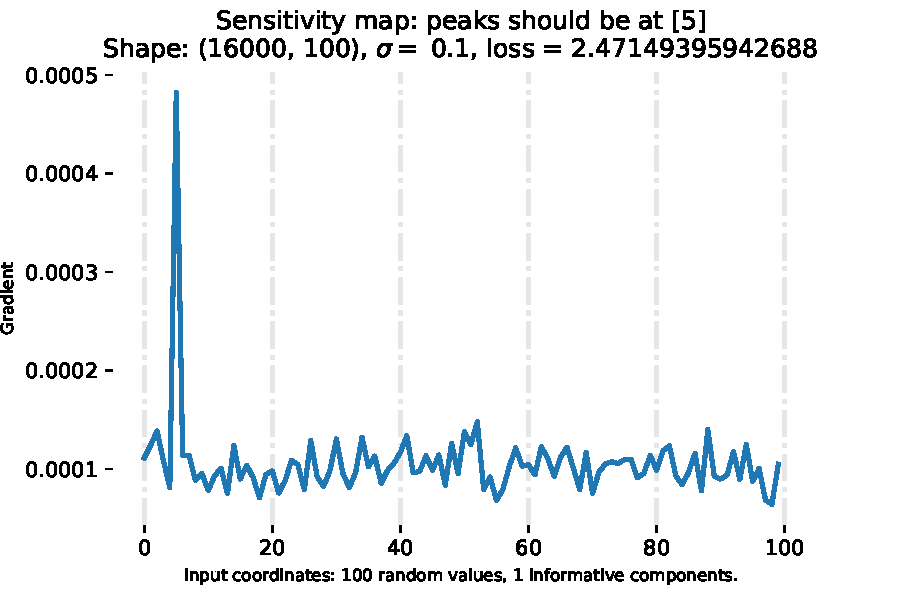
\includegraphics[width=\textwidth]{figures/experience_1/1_shares_shape_16000_100_30_n_hidden_0_dot_1_sigma}
		\caption{One share}
		\label{fig:toy_example_1}
	\end{subfigure}
	\begin{subfigure}{0.49 \textwidth}
		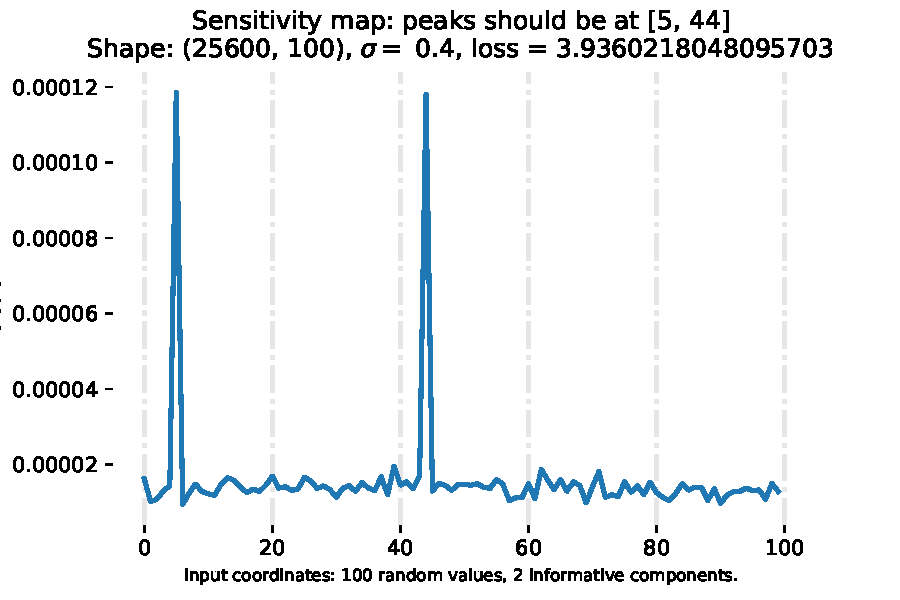
\includegraphics[width=\textwidth]{figures/experience_1/2_shares_shape_25600_100_30_n_hidden_0_4_sigma}
		\caption{Two shares}
		\label{fig:toy_example_2}
	\end{subfigure}
	\begin{subfigure}[]{0.49 \textwidth}
		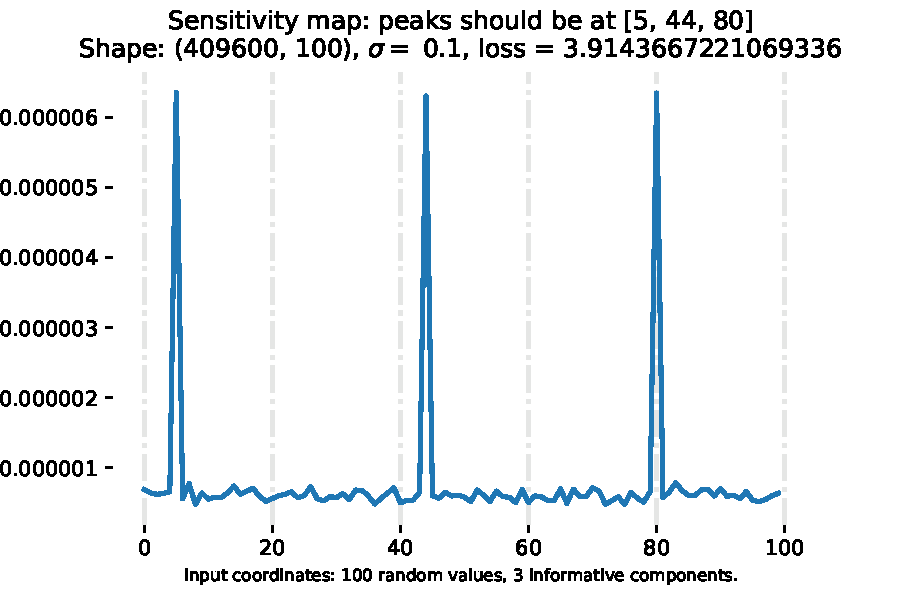
\includegraphics[width=\textwidth]{figures/experience_1/3_shares_shape_409600_100_100_n_hidden_0_1_sigma}
		\caption{Three shares}
		\label{fig:toy_example_3}
	\end{subfigure}
	\caption{Gradient of the loss function, averaged over the validation traces.}
	\label{fig:toy_example}
\end{figure} 
\autoref{fig:toy_example} presents some examples obtained for 1 (\autoref{fig:toy_example_1}), 2 (\autoref{fig:toy_example_2}) and 3 (\autoref{fig:toy_example_3}) shares. 
We clearly see some peaks at the coordinates where the meaningful information have been placed.
This confirms that our characterization method is sound when facing leakages protected by secret-sharing, no matter the order though it required \(16\) times more simulated data and less noised data (\(\sigma^2 \geq 0.1\)) than for the same experiment against first order secret-sharing.


\subsection{Comparison with SNR for Characterization}
\label{sec:related_works}
Now we have shown that \gls{gv} is relevant for characterization on simulated data, one may wonder to what extent this method would be useful compared to other characterization techniques.
In this section, we compare our contribution to the \gls{snr} used for \glspl{poi} selection, as presented in \autoref{sec:characterization}.

One has to keep in mind that the \gls{snr} is a statistical tool, and produces a single characterization from all the profiling traces; whereas our method gives one map for each trace, though we might average them.
This observation has two consequences.
First, if an \gls{snr} characterization is launched in presence of secret-sharing, every trace coordinate \(\XXX[t]\) is likely to be independent from \(\Z\), which will lead the numerator of the \gls{snr} (\autoref{eq:SNR}) to converge towards \(0\).
Secondly, if an \gls{snr} characterization is launched in presence of de-synchronization, then the denominator of \autoref{eq:SNR} is expected to be multiplied by the maximum shift, as argued in \autoref{sec:hiding}.
To sum-up, an \gls{snr} characterization cannot directly highlight higher order leakages when the random material -- used for secret-sharing and/or for de-synchronization -- is not assumed to be known.
Some solutions to deal with this issue have been proposed, \eg{}, by pre-processing the traces with some re-combination functions -- see \autoref{sec:characterization} -- or by applying realignment techniques~\cite{van_woudenberg_improving_2011,nagashima_dpa_2007,durvaux_efficient_2012}.


\subsection{Related Works}
\label{sec:biblio_cosade}
The idea of using the derivatives of differentiable models to visualize information is not new. 
Following the emergence of deep convolutional networks, Simonyan \etal~\cite{simonyan_deep_2013} have first proposed the idea of \gls{gv} to generate a so-called \emph{Sensitivity Map} for image recognition.
The approach was motivated by the fact that such a map can be computed for free thanks to the back-propagation algorithm.
A derived method, called \emph{Guided Backpropagation} has also been proposed by Springenberg \etal{}~\cite{springenberg_striving_2014}.
The latter one slightly modifies the back-propagation rule in a \gls{relu} layer in order to filter the contributions from the upper layers.
Actually, Montavon \etal{}~\cite{montavon_methods_2018} state that visualizing the gradient only tracks an explanation to the variation of a final decision -- \(\MLmodel(\xxx, \MLparam)\) in our context -- and
not directly the decision itself.
To circumvent this, they propose a visualization method called \gls{lrp}.
Another method called \emph{Deconvolution} has been proposed by Zeiler \etal{}~\cite{zeiler_visualizing_2013} in order to give insights about the regions of an input data contributing to the activation of a given feature in a model (either in an intermediate layer or in the output layer).
In the field of Image Recognition, these methods have been shown to be more relevant than \gls{gv}.

However, the \gls{sca} and Image Recognition fields differ.
In the latter one, the decision is highly diluted among lots of pixels, and the decision surface might be locally flat, though we are in an area of interest.
Hopefully in an \gls{sca} context, \autoref{assum:sparsity} states that it is reasonable to consider that the information is very localized.  
That is why we are in a particular case where looking at the output sensitivity may be at least or even more interesting than other visualization methods.

In parallel to the publication of our paper at \textsc{Cosade} 2019, Timon has proposed at \textsc{Ches} 2019 the same method, under the name of sensitivity analysis~\cite{timon_non-profiled_2019}.%
\footnote{
	We prefer using the term ``gradient visualization'' rather than ``sensitivity analysis'' which is a metonymy: the latter one encompasses the former one, beside other techniques.
}
Likewise, Hettwer proposed at \textsc{Sac}'19 a comparison between several techniques such as the \gls{gv}, the \gls{lrp}, and some occlusion techniques~\cite{hettwer_deep_2019}.
The latter ones consist in removing some areas of an input trace, in order to study how a trained model reacts in its predictions.
A relevant area should therefore lead to strong dissimilarities in the corresponding predictions when it is removed.
Later, Zaid \etal{} proposed the use of \emph{heatmaps}~\cite{zaid_methodology_2019}.%
\footnote{Another technique used by the authors, called \emph{weight visualization} is rather focused on the understanding of the learned weights of the dense layers in a \gls{cnn}, therefore beyond the scope of this study.}
It consists in computing the average output over all filters of a given convolution layer.
In particular, the heatmap of the first layer is expected to produce a similar map as the \gls{gv}.
Wouters \etal{}, in a paper revisiting the results of Zaid \etal{}, used a variant of the \gls{gv} called \emph{Gradient \(\times\) Input} consisting in multiplying the map returned by \gls{gv} with the input trace itself~\cite{wouters_revisiting_2020}.
Likewise, Van der Valk \etal{} have investigated the \emph{Singular Vector Canonical Correlation Analysis} provide insights on the layers of a trained \gls{mlp}~\cite{vanDerValk_kilroy_2019}.
Finally, Bursztein \etal{} presented at \textsc{Defcon} 2020 a tool involving explainability techniques for \gls{dl} similar to \gls{gv}~\cite{elie_scadl_2020}.
By using characterization maps similar to the ones produced by the \gls{gv} method, they are able to produce a mapping with the assembly instructions yielding the informative leakage.
Thanks to a reverse-engineering tool, they are able to map the leaky assembly instructions to the corresponding area in the code, enabling to precisely identify the vulnerability.